\section{Project Results}

\subsection{Upgrade Dependencies}

\begin{frame}[c]
    From Django 2 to Django 3 \\
    (Django 4 released during the project, has been decided to go to 3 in production first)
\end{frame}

\subsection{Proper Logging}

\pic{Logging Now}{31}

\begin{frame}[c]{Logging Now}
    \large
    \begin{itemize}[<+(1)->]
        \item Properly defined Logging levels (debug, info, warn, error, critical)
        \item Logging to console, syslog and file
        \item Differing formatter for console and other (timestamps, ...)
        \item Rotating files: Keep last five days, overwrite after
    \end{itemize}
\end{frame}

\subsection{Attempt to automatically generate documentation}

\begin{frame}[c]{Automatically Generate Documentation}
    \begin{multicols}{2}
        \large
        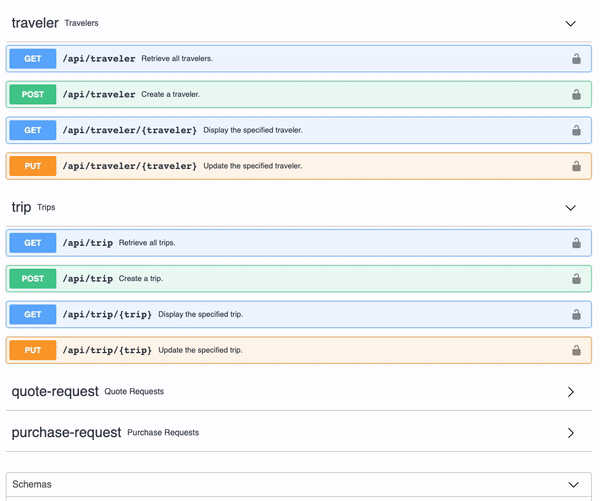
\includegraphics[width=0.5\textwidth]{swagger} \\
        (Example) \\
        Failed, because:
        \begin{itemize}[<+(1)->]
            \item Mainly used to generate documentation for JSON endpoints
            % \item Few comments to generate documentation from
            \item 'Primitive' Views lacking important information for automatic generation
        \end{itemize}
        Was worth a try.
    \end{multicols}
\end{frame}

\subsection{Selecting a DFG board}

\begin{frame}[c]{Excerpt of DFG subject areas}
    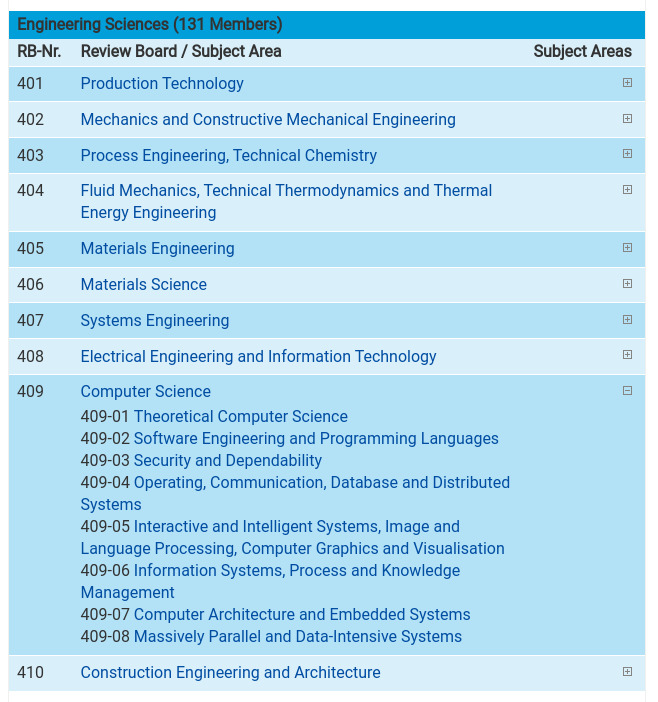
\includegraphics[height=\textheight]{Selection_032}
\end{frame}
\pic{Selection of DFG Subject Area upon Project Creation}{10}


\begin{frame}[c]{Selection of DFG Discipline}
    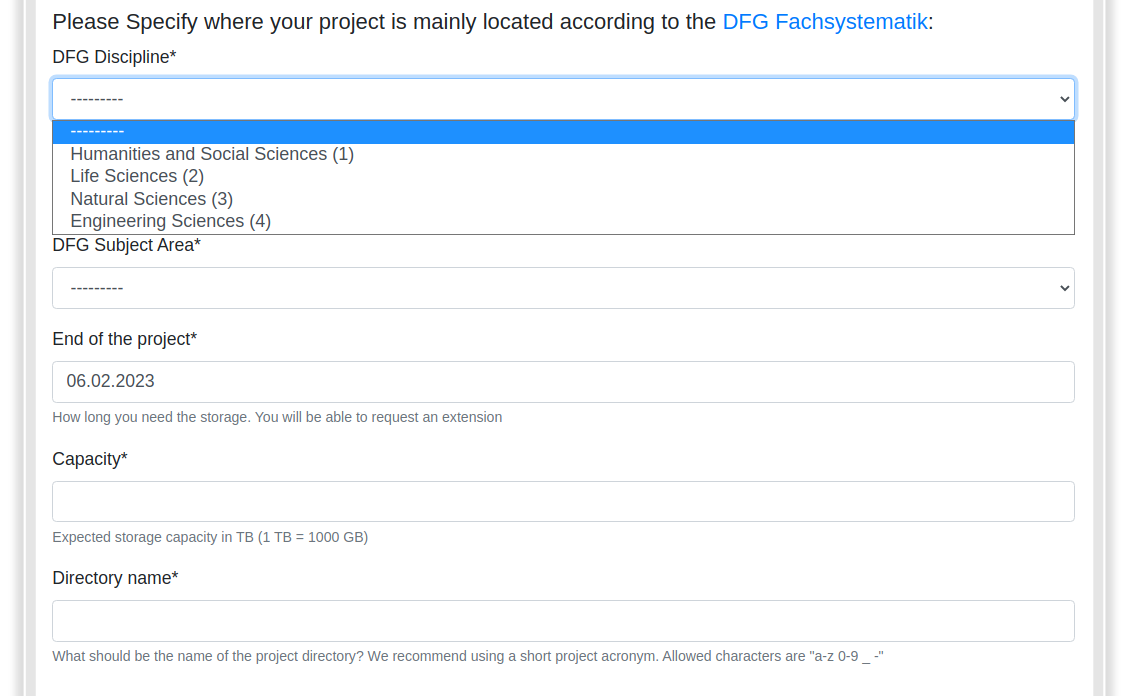
\includegraphics[width=\textwidth]{select_discipline}
\end{frame}
\begin{frame}[c]{Selection of DFG Subject without Board}
    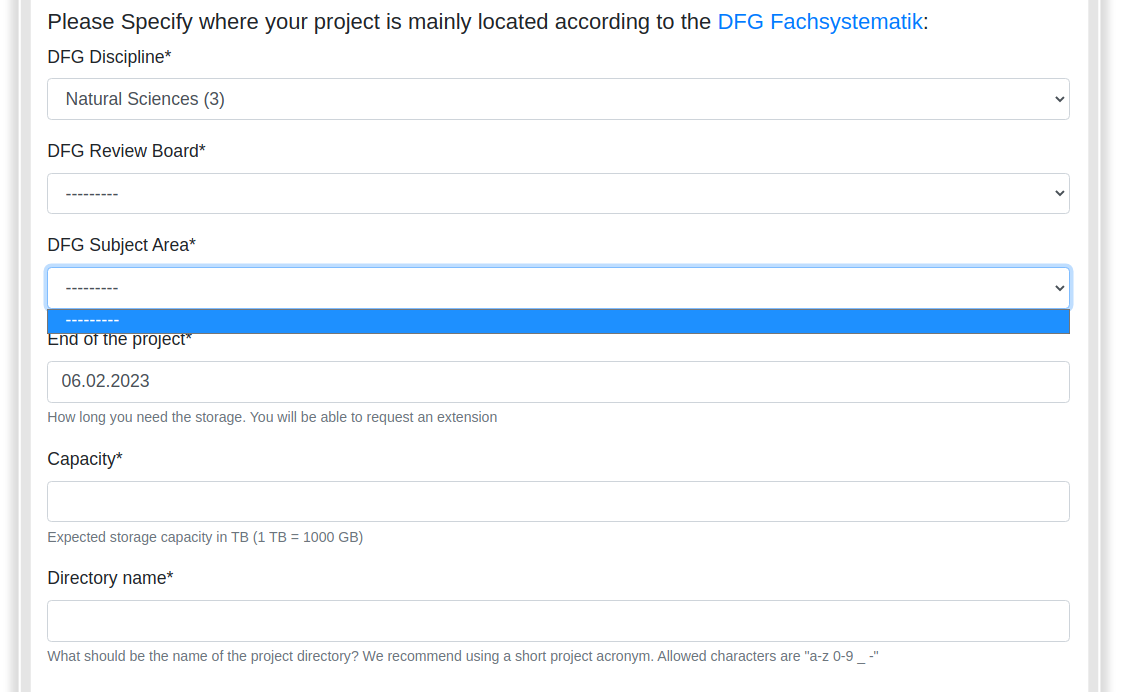
\includegraphics[width=\textwidth]{select_subject1}
\end{frame}
\begin{frame}[c]{Selection of DFG Subject}
    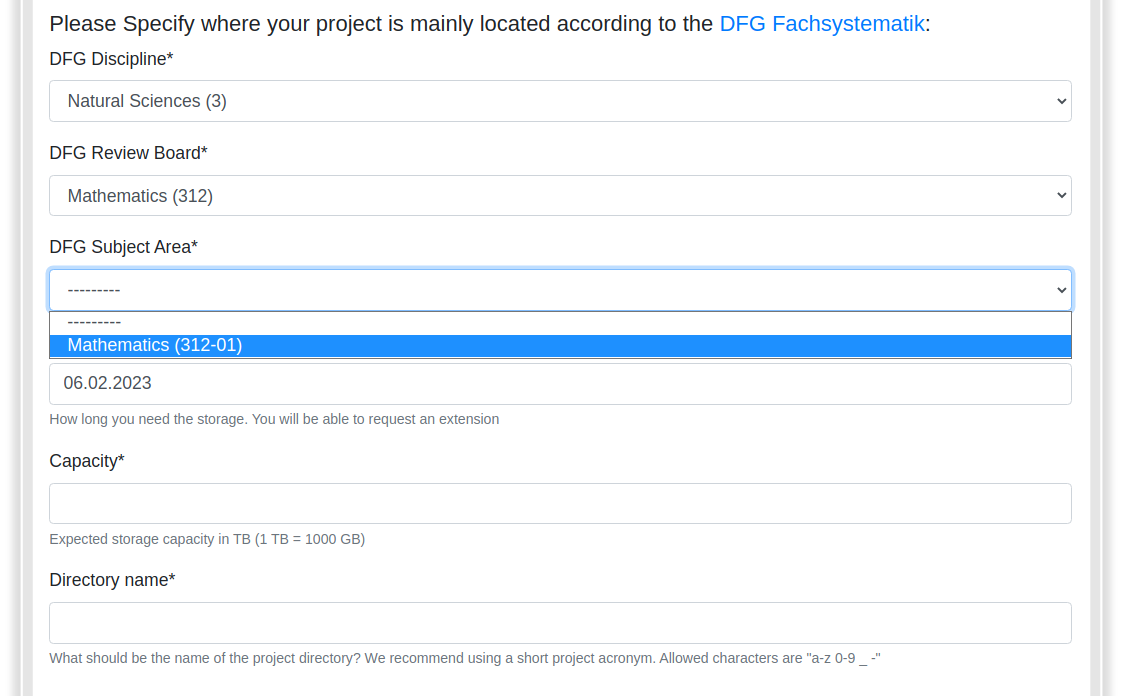
\includegraphics[width=\textwidth]{select_subject2}
\end{frame}


\begin{frame}[c]{Code}
    \todo{code of change function with request}
    \todo{maybe from other side as well?}
\end{frame}

%     \$("#id_board").change(function () \{
%       /* on change of board field, request new data for `field` field */
%       var url = \$("#form").attr("data-fields-url");
%       var board = \$(this).val();
% 
%       \$.ajax(\{
%         url: url,
%         data: \{
%           'board': board
%         \},
%         success: function (data, textStatus, jqXHR) \{
%           \$("#id_field").html(data);
%         \}
%       \});
% 
%     \});


% \begin{frame}[c]
%     Next project: implement analytics page showing used capacity by area. \\
%     \todo{Picture of callback from page to select available from database} \\
%     \todo{Show parts of the code}
% \end{frame}

\subsection{Diff to schema in database}

\begin{frame}[c]{The DFG schema changes frequently}
    \large
    \begin{itemize}[<+(1)->]
        \item The DFG schema changes every four years
        \item It was last changed in 2020
        \item So it'll change again in two years
        \item Not clear how much (probably not a whole lot)
    \end{itemize}
    \pause
    So I implemented a command to compare any csv to what is currently in the database:
    \todo{code listing}
\end{frame}


% \subsection{Rename Models}
% 
% \begin{frame}[c]
%     % Order -> LSDFProject
%     % PersonOrder -> ProjectRole
%     % ...
%     Worked quite well, generated some migrations
% \end{frame}

% \subsection{Attempt to rename entire App}
% 
% \begin{frame}[c]
%     Failed, ultimately unclear why, requires deep django/database knowledge.
% \end{frame}


\subsection{Attempt to properly modularize PersonForm}

\begin{frame}[c]
    Explain the problem (show exemplary code) of redundancy
    Managed to get quite far, very good (deep) learning example, and absolutely
    possible. just requires some more time than expected.
    Nags me that it's not modular yet. Some day.
\end{frame}


\subsection{Extension Requests}

\begin{frame}[c]{Extension Requests}
    Much-requested feature.
    \todo{Overview of newly introduced routes, views, forms, models and relations}
\end{frame}




% \subsection{Relative to Absolute Imports}
% 
% \begin{frame}[c]
%     Very early on, succeeded
% \end{frame}


